\chapter{Introduzione alla programmazione lineare a numeri interi}

Si consideri il seguente problema.
\begin{flalign}
	& Min\;cx \\
	& \;\;\;\;\;\;\;Ax=b \\
	& \;\;\;\;\;\;\;x\ge 0 \\
	& \;\;\;\;\;\;\;x\;intero
\end{flalign}
Le variabili devono assumere valori interi:
\begin{flalign}
	& Es:\;\;x_{i}=Numero\;di\;uomini\;che\;devono\;essere\;assegnati\;al\;lavoro\;i. \\
	& \;\;\;\;\;\;\;\;\;\;\;\;\;=Numero\;di\;automezzi\;che\;devono\;operare\;il\;trasporto\;lungo\;la\;"tratta\; i". \\
\end{flalign}

\section{Arrotondamento ad una soluzione non-intera}
Si risolva il problema ignorando i vincoli [$x: intero$].
Le variabili che risultano non intere, nella soluzione ottima del problema continuo, vengano arrotondate al valore intero pi\`u vicino.
\begin{flalign}
	& Es:\;\;Min\;z=-2x_{1}+3x_{2} \\
	& \;\;\;\;\;\;\;\;\;\;x_{1}+x_{2}\ge 3 \\
	& \;\;\;\;\;\;\;\;\;\;3x_{1}+x_{2}\le 6 \\
	& \;\;\;\;\;\;\;\;\;\;x_{2}\le 5 \\
	& \;\;\;\;\;\;\;\;\;\;x_{1},\;x_{2}\ge 0\;ed\;intere
\end{flalign}
\begin{figure}[h]
	\centering
	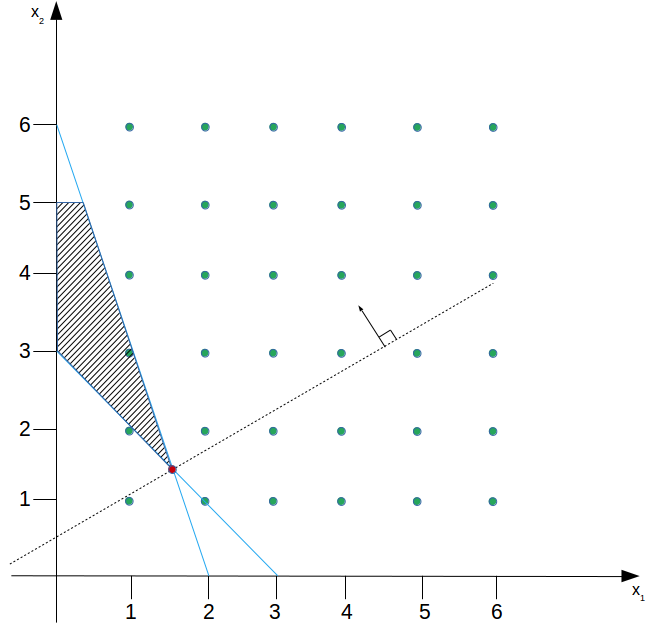
\includegraphics[height=12cm]{images/graph6.png}
	\label{fig:SoluzioneOttimaContinua1}
	\caption[]{\\Soluzione continua: $z=\frac{3}{4}$; $x_{1}=\frac{3}{2}$, $x_{2}=\frac{3}{2}$ \\ Soluzione intera: $z=4$; $x_{1}=1$, $x_{2}=2$}
\end{figure}

In questo esempio la soluzione arrotondata coincide con la soluzione ottima.

\begin{flalign}
& Es:\;\;Min\;z=8x_{1}+6x_{2} \\
& \;\;\;\;\;\;\;\;\;\;4x_{1}+3x_{2}\ge 6 \\
& \;\;\;\;\;\;\;\;\;\;x_{1},\;x_{2}\ge 0\;ed\;intere
\end{flalign}
\begin{figure}[h]
	\centering
	\captionsetup{justification=centering}
	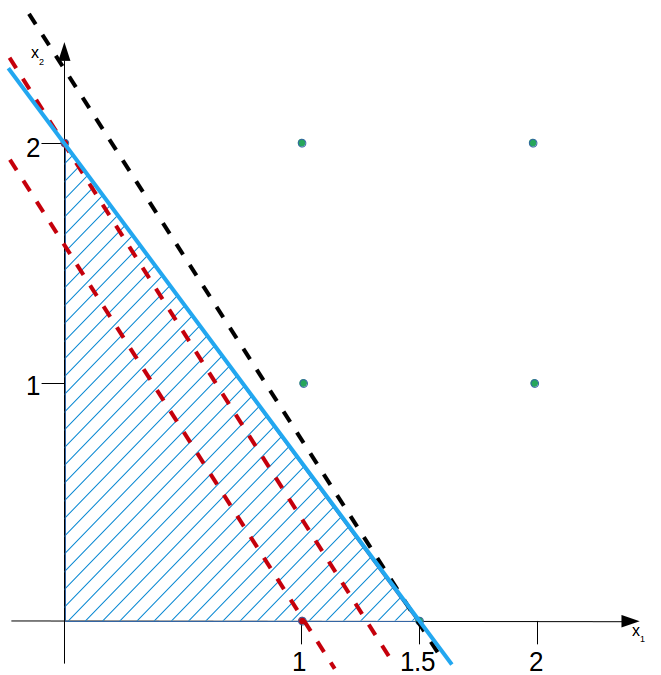
\includegraphics[height=13cm]{images/graph7.png}
	\label{fig:SoluzioneOttimaContinua2}
	\caption[]{\\ Soluzione continua: $z=12$; $x_{1}=1,5$, $x_{2}=0$ \\ Soluzione arrotondata $z=8$; $x_{1}=1$, $x_{2}=0$ \\ Soluzione intera: $z=10$; $x_{1}=0$, $x_{2}=2$}
\end{figure}

La soluzione arrotondata si discosta notevolmente dalla soluzione ottima.

\begin{flalign}
& Es:\;\;Min\;z=8x_{1}+6x_{2} \\
& \;\;\;\;\;\;\;\;\;\;4x_{1}+3x_{2}\ge 6 \\
& \;\;\;\;\;\;\;\;\;\;x_{1},\;x_{2}\ge 0\;ed\;intere
\end{flalign}
\begin{figure}[h]
	\centering
	\captionsetup{justification=centering}
	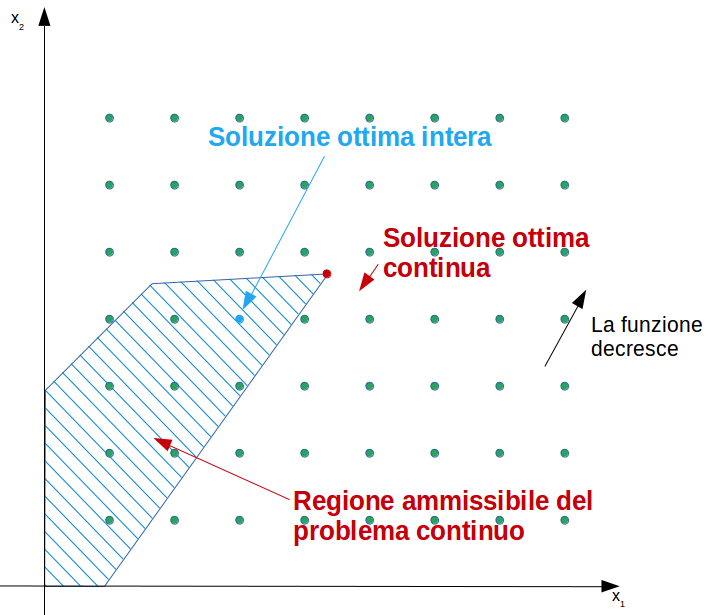
\includegraphics[height=13cm]{images/graph8.png}
	\label{fig:SoluzioneOttimaContinua3}
\end{figure}

I quattro punti interi pi\`u vicini alla soluzione continua non sono ammissibili.